%% LyX 2.3.6 created this file.  For more info, see http://www.lyx.org/.
%% Do not edit unless you really know what you are doing.
\documentclass[aps,prl,twocolumn,superscriptaddress,showpacs]{revtex4-1}
%%%%%%%%%%%%%%%%%%%%%%%%%%%%%%%%%%%%%%%%%%%%%%%%%%%%%%%%%%%%%%%%%%%%%%%%%%%%%%%%%%%%%%%%%%%%%%%%%%%%%%%%%%%%%%%%%%%%%%%%%%%%%%%%%%%%%%%%%%%%%%%%%%%%%%%%%%%%%%%%%%%%%%%%%%%%%%%%%%%%%%%%%%%%%%%%%%%%%%%%%%%%%%%%%%%%%%%%%%%%%%%%%%%%%%%%%%%%%%%%%%%%%%%%%%%%
\usepackage{amsmath}
\usepackage[UTF8]{ctex}
\usepackage{graphicx,graphics}
\usepackage{hyperref}
\usepackage{amssymb}
\usepackage{color}
\usepackage{appendix}
\usepackage{lipsum}
\usepackage{physics}
\usepackage{fancyhdr}
\usepackage{background}
\setcounter{MaxMatrixCols}{10}



\backgroundsetup{scale=1, angle=0, opacity = 0.1,
contents = {
\includegraphics[width=\paperwidth, height=\paperwidth, keepaspectratio]{background.pdf}}}

%页眉页脚设置
\setlength{\headheight}{29.46504pt}
\fancyhead[L]{} %%留空则不显示
\fancyhead[C]{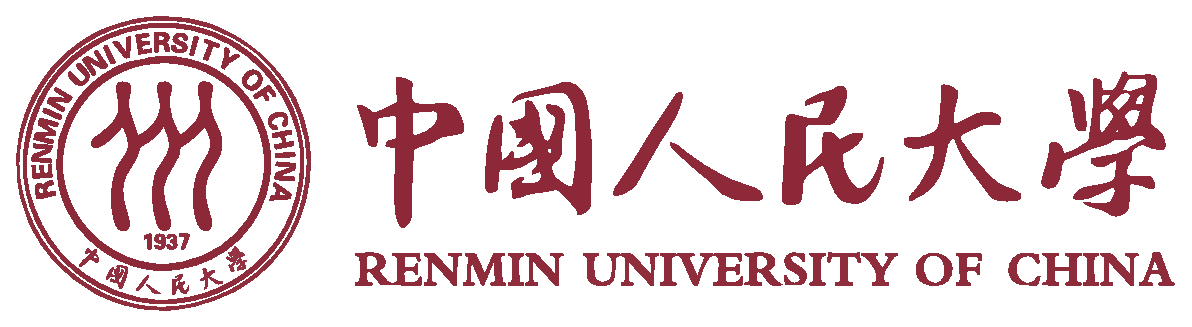
\includegraphics[width=0.2\linewidth]{Renmin_Univ_Logo.eps}} %%留空则不显示
\fancyhead[R]{物理实验报告} %%留空则不显示
\fancyfoot[L]{}
\fancyfoot[R]{中国人民大学物理实验中心\ \ }
\fancyfoot[C]{ \thepage }
\pagestyle{fancy}

\begin{document}
\begin{figure}
    \centering
    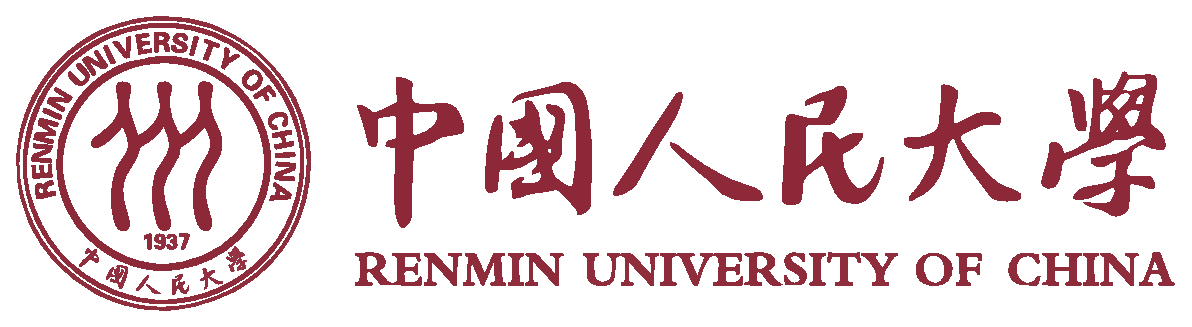
\includegraphics[width=0.6\linewidth]{Renmin_Univ_Logo.eps}
\end{figure}
\title{\LARGE 物理实验报告}%实验题目
\author{\large 陈小赫}%姓名
\thanks{本次实验的指导老师为:谭小云}%指导老师
\affiliation{中国人民大学物理学系2022200XXX}%学号
\date{2024年2月30日}%实验日期
\begin{abstract}
    %这里是你的摘要,对实验主要内容进行简明扼要的介绍,包括研究目的、方法、结果和结论,通常在100-300字之间。
    %\lipsum用以生成随机文本,实际使用时删除即可
\lipsum[1]
\end{abstract}
\maketitle
\textbf{\large I 引言:}\vspace{0.3cm}

%引言
\lipsum

\vspace{0.3cm}\textbf{\large II. 方法:}\vspace{0.3cm}

\lipsum

\vspace{0.3cm}\textbf{\large III. 结果:}\vspace{0.3cm}

\lipsum

\vspace{0.3cm}\textbf{\large IV. 结果}\vspace{0.3cm}

\lipsum

this is citation\cite{Mitra-16}
\begin{widetext}
    \lipsum[2]
\end{widetext}

\vspace{0.3cm}\textbf{\large V. 讨论}\vspace{0.3cm}

\lipsum


\vspace{0.3cm}\textbf{\large V. 结论}\vspace{0.3cm}


\begin{thebibliography}{10}
   
    \bibitem{Mitra-16}D. Mitra, P. T. Brown, P. Schau\ss{}, S. S. Kondov, and W. S. Bakr, Phys. Rev. Lett. \textbf{117}, 093601 (2016).
    
\end{thebibliography}

\end{document}
